\documentclass[a4paper,11pt]{article}

\usepackage[french]{babel}
\usepackage[T1]{fontenc}
\usepackage[utf8]{inputenc}
\usepackage{lmodern}
\usepackage{graphicx}
\usepackage{fancyhdr}
\usepackage{amssymb}
\usepackage{geometry}
\usepackage{lastpage}
\usepackage[dvipsnames]{xcolor}
\usepackage{hyperref}
\usepackage{textcomp}
\usepackage{hyperref}

\geometry{hmargin=2cm}

\title{SO ETNA \\ Prise en main}
\author{TRAN BA Philippe , TRAORE Abdoulaye , REBUFFET Jean-Baptiste \\ ETNA promo 2018}

\begin{document}

\pagestyle{fancy}
\date{}
\chead{}
\rhead{}
\lfoot{TRAN BA Philippe , TRAORE Abdoulaye , REBUFFET Jean-Baptiste}
\cfoot{}
\rfoot{Page \thepage\ sur \pageref{LastPage}}
\renewcommand{\headrulewidth}{0.4pt}
\renewcommand{\footrulewidth}{0.4pt}

\maketitle
\tableofcontents

\vspace{2 cm}

\section*{Préface}

Ce document indique comment se connecter au serveur SO ETNA et d'en exploiter les fonctionnalités les plus basiques
et les plus importantes. Il ne contient en aucun cas toutes les fonctionnalités avancées incluses dans la version actuelle.

\newpage

\section{Comment se connecter}

Pour se connecter, il suffit d'ouvrir dans son navigateur web favori l'URL du serveur. Dans notre cas, ce sera très probablement
\url{SOETNA.etna-alternance.net}. Une fois le lien ouvert, la page ci-dessous apparaitra. L'identifiant qu'on utilisera
sera le couple admin et password. Le mot de passe d'admin devra être rapidement modifié pour des raisons de sécurité évidentes.

\vspace{1 cm}

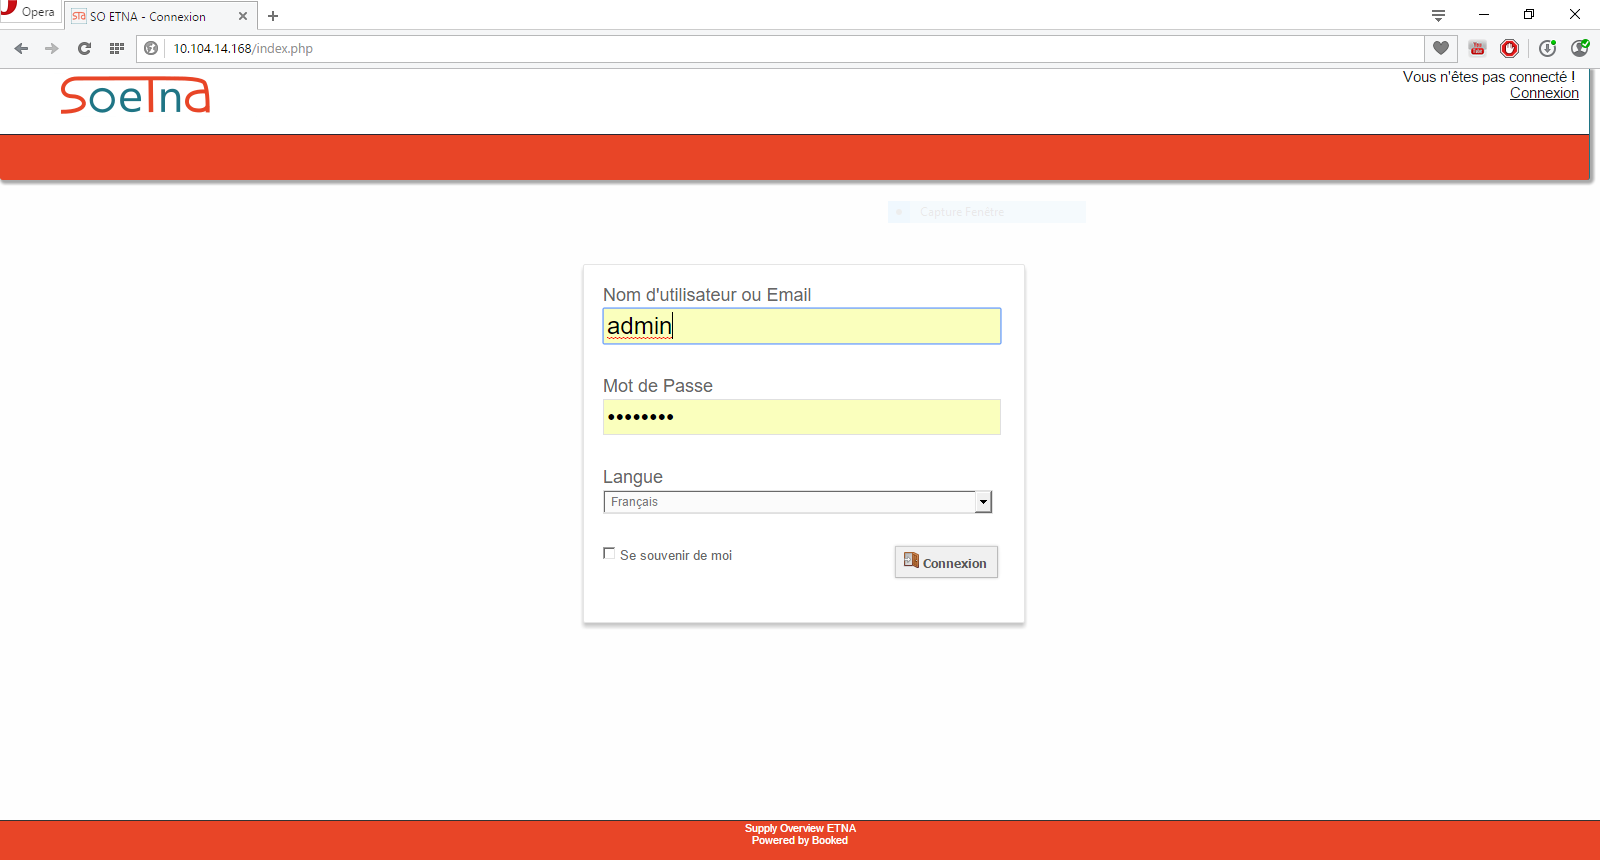
\includegraphics[width=15cm]{./login.PNG}

\newpage

\section{Création d'une ressource}

\subsection{Qu'est-ce qu'une ressource ?}

Une ressource est un item, que ce soit un appareil ou une salle que les utilisateur pourront emprunter ou occuper.
Chaque ressource aura son propre agenda ainsi que des descriptions et autres paramètres. Elle aura entre autre comme sur l'image plus bas :

\begin{itemize}
 \item Une image, une petite photo est bien plus parlante que de longues phrases.
 \item Un statut, désignant si la ressource est disponible ou non en ce moment.
 \item Un planning, désignant sur quel calendrier la ressource apparaitra.
 \item Un type, qui définit le type de la ressource, si c'est une salle ou un écran. Ce paramètre sert à trier les ressources
 \item Un numéro, qui sert à trier les ressources aussi. Par défaut SOETNA classera les ressources par ordre croissant et la valeur par défaut est 0.
 \item Un emplacement, qui détermine dans quelle salle ou étagère trouver la ressources.
 \item Un contact, qui sert de référent pour cette ressource.
 \item Une description, qui précise la ressource.
 \item Une note, qui peut par exemple préciser l'usure du matériel.
 \item Un administrateur de ressource, qui détermine la personne qui autorisera ou non le prêt.
\end{itemize}

\vspace{1 cm}

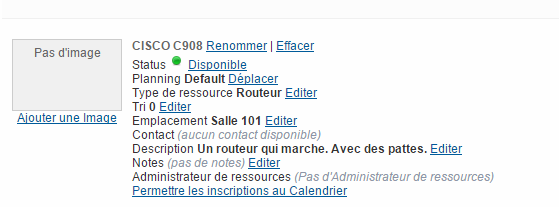
\includegraphics[width=15cm]{./res3.PNG}

\vspace{1 cm}

Aucun de ces paramètres n'est obligatoire et ceux qui le sont ont une valeur par défaut correcte dans la plupart des cas.

Pour résumer l'affichage qui peut être filtré à l'aide du menu a gauche, les ressources sont triées dans
l'ordre croissant de leur numéro puis dans l'ordre alphabétique.

\newpage

\subsection{Comment créer une ressource ?}

Pour créer une ressource, il faut aller dans l'onglet "Gestion de l'application" puis cliquer sur "Ressources". Il ne faut PAS cliquer sur les sous-menus
de ressource.

\vspace{1 cm}

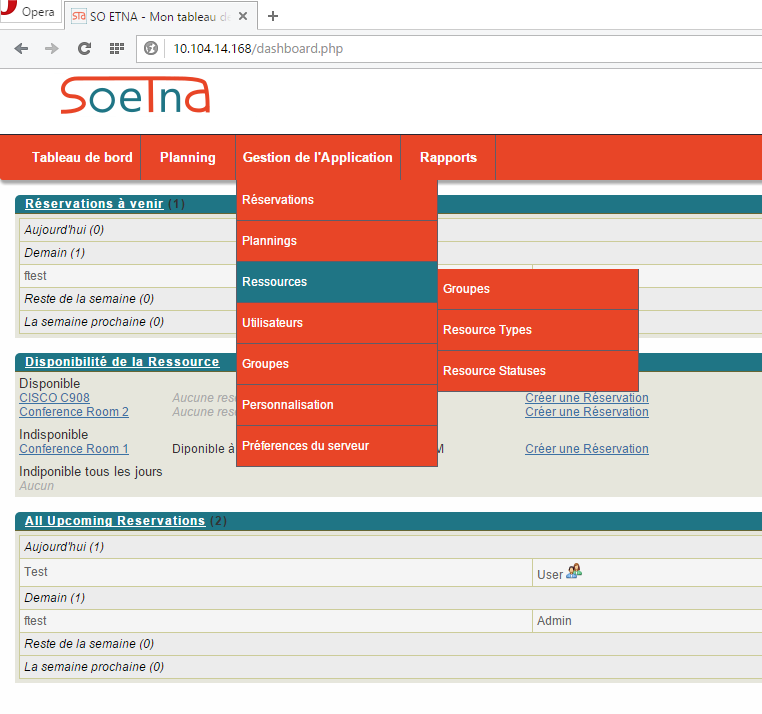
\includegraphics[width=15cm]{./res1.PNG}

\newpage

Ensuite, tout en bas de la page, il y a la section "Ajouter une nouvelle ressource". Dans cette section, entrez juste le nom de la ressource 
et cliquez sur "Ajouter une ressource". Tous les paramètres sont à modifier si besoin ultérieurement.

\vspace{1 cm}

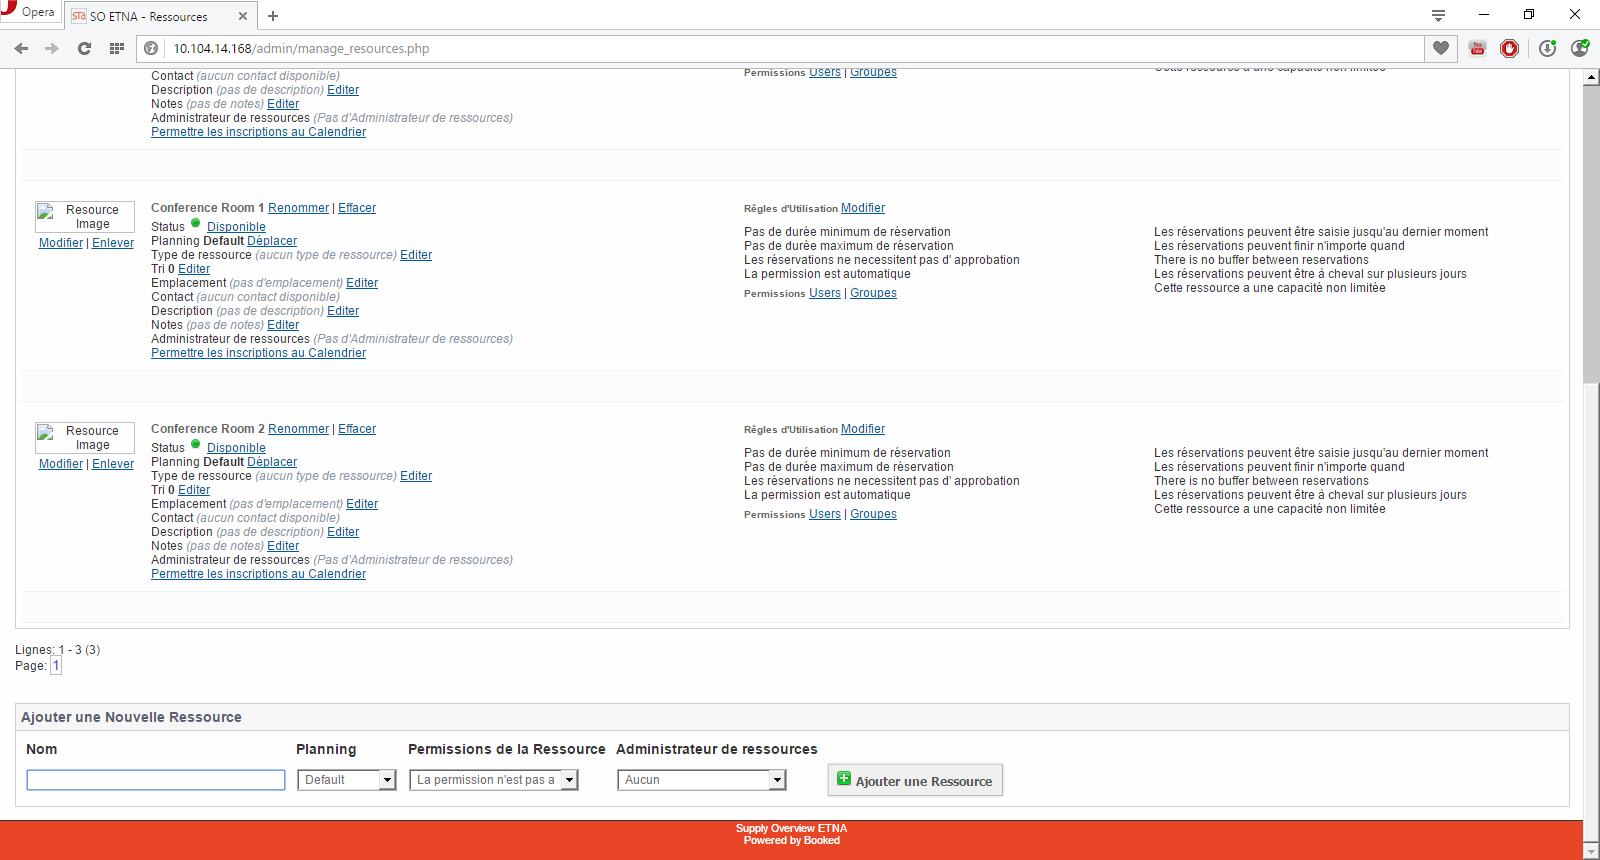
\includegraphics[width=15cm]{./res2.PNG}

\vspace{1 cm}

Et voilà, votre ressource est créée. Elle devrait à présent être affichée dans la liste. Si elle n'y est pas, vérifiez les filtres.

\newpage

\section{Réservation d'une ressource}

\subsection{Disponibilité d'une ressource}

Pour accéder au calendrier de réservation des ressources, il faut cliquer sur l'onglet "planning"
Un calendrier apparaitra, avec une ligne par ressources. Pour rappel, il est possible d'alléger l'affichage
en filtrant les ressources que l'on veut afficher via la liste déroulante sur la gauche. Dans notre exemple ci dessous, nous n'affichons que
le type routeur que nous avons créé pour notre batterie de test. Il n'existe qu'une unique ressource de type routeur.
Donc seule celle-ci est affichée.

\vspace{1 cm}

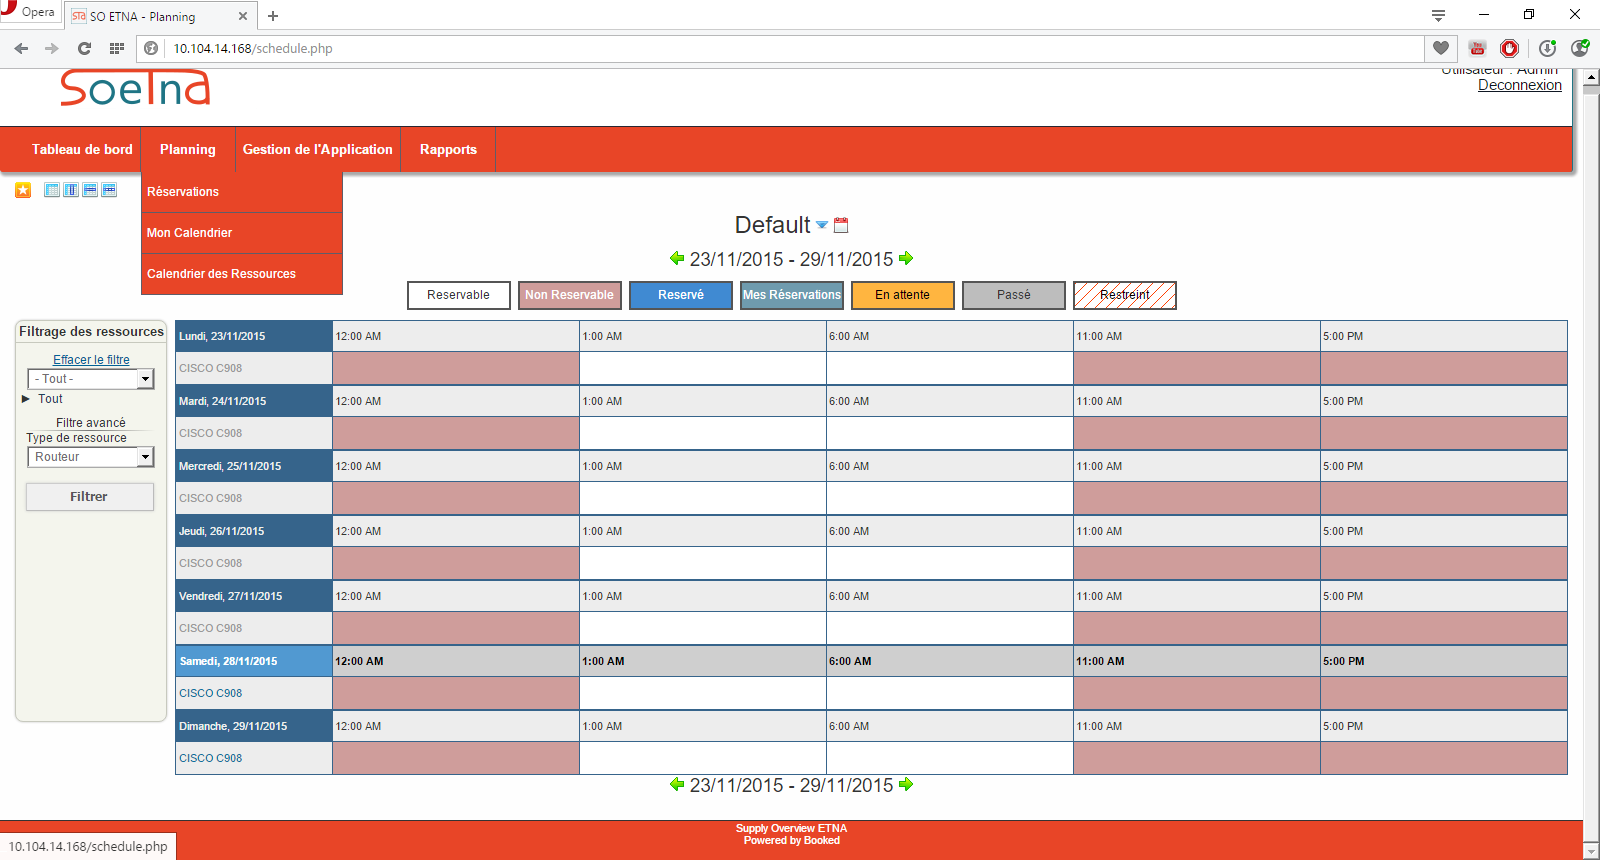
\includegraphics[width=15cm]{./resa1.PNG}

\vspace{1 cm}

On voit ici que notre ressource de type routeur nommée CISCO C908 est disponible toute la semaine du 23/11/15 au 29/11/15.
Le nombre et la largeur des plages horaires peut être modifiée dans un autre menu.

\newpage

Dans la capture ci-dessous, on voit que la ressource est allouée à l'utilisateur sur cette page, c'est à dire nous. Dans le cas où la ressource serait indisponible, elle serait affichée en bleu clair sur
les plages horaires adéquates.

\vspace{1 cm}

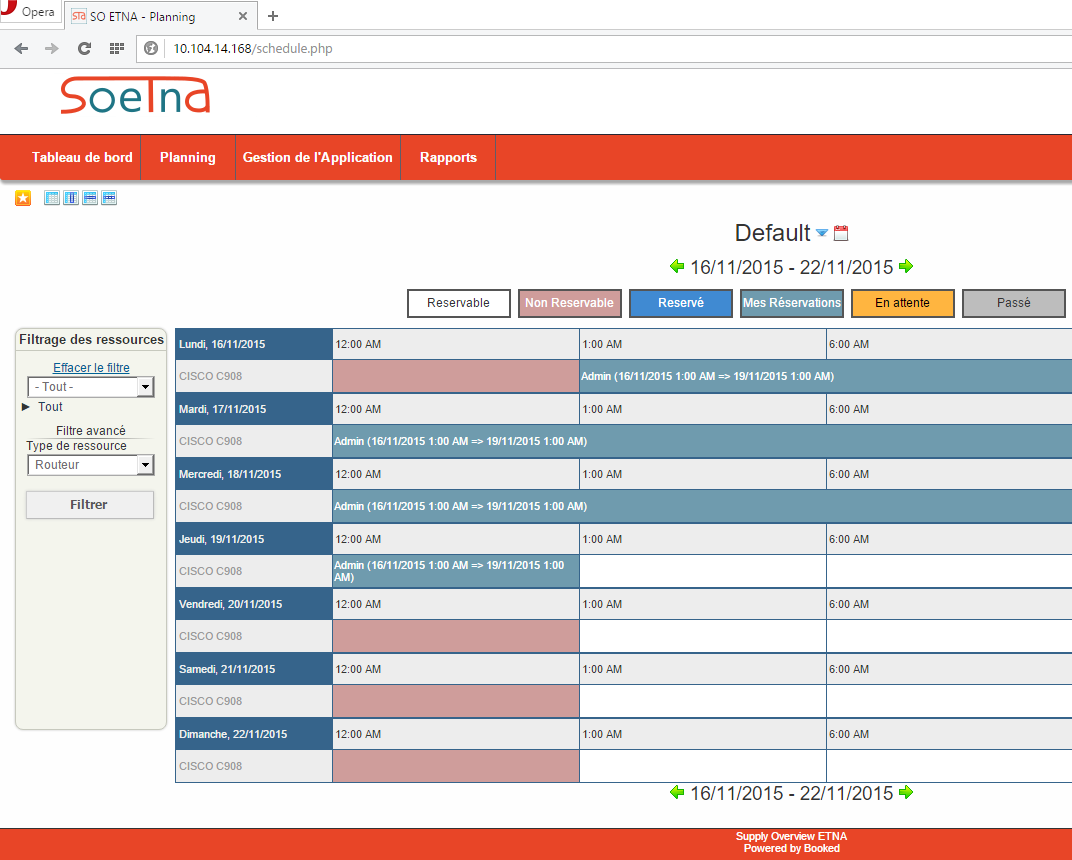
\includegraphics[width=15cm]{./resa3.PNG}

\newpage

\subsection{Réservation}

Pour réserver une ressource, il suffit de cliquer sur une plage horaire, de préférence, celle de début de l'emprunt.
Le menu ci-dessous s'affichera et il suffira d'indiquer la début et la fin de 
la période d'emprunt. Les autres paramètres étant optionnels, nous cliquons sur le bouton "créer".

\begin{center}
	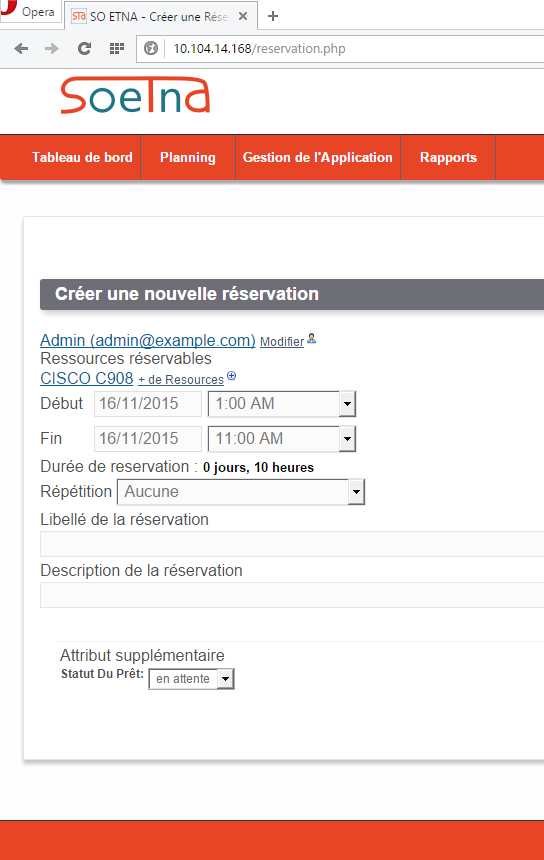
\includegraphics[height=15cm]{./resa2.PNG}
\end{center}

\vspace{1 cm}

La ressource est potentiellement réservée à présent. Elle l'est directement si aucune personne
n'est censée valider la demande de réservation. Sinon, elle est en attente ou peut être refusée
par l'administrateur de la ressource.

\newpage

\section{Définir un type}

Le type d'une ressource est un paramètre très pratique d'une ressource. Il permet de trier et de retrouver facilement une ressources ou alors des ressources équivalentes. Par exemple, dans le cas d'emprunt d'une salle -de type salle donc-, l'emplacement et le nom de la salle ne sont pas toujours important et l'on cherche donc simplement parmi toutes les salles une salle disponible.

Pour créer un type de ressources, il faut aller dans l'onglet "Gestionnaire de l'application" puis dans "Ressource" et cliquer sur le sous-menu "Ressources types" :

\vspace{1 cm}

\begin{center}
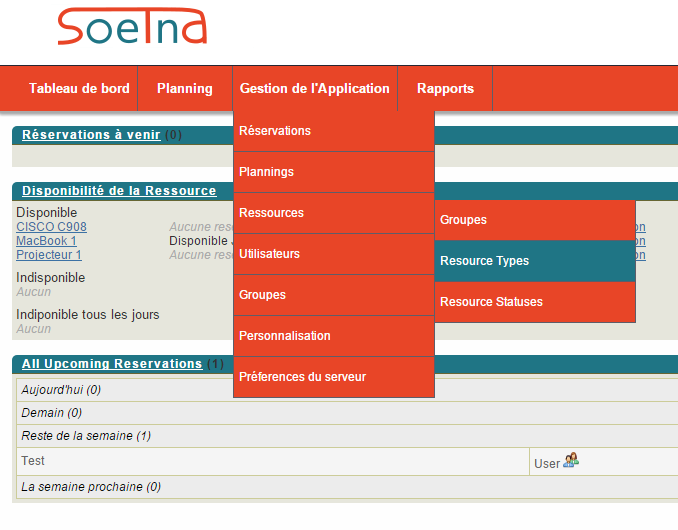
\includegraphics[height=11cm]{./grp1.PNG}
\end{center}

\vspace{1 cm}

La page suivante s'affiche et il suffit d'entrer le nom du type que l'on souhaite créer ainsi qu'une description optionnelle.

Pour affecter des ressources dans un type, il faut retourner dans le menu des ressources puis d'éditer le type des ressources souhaité.

\end{document}